
%<<setup-child, include = FALSE>>=
%library(knitr)
%set_parent("../style/preamble.Rnw")
%@

\input{../../2021/style/preamble4tex}
% dependencies: amsmath, amssymb, dsfont
% math spaces
\ifdefined\N
\renewcommand{\N}{\mathds{N}} % N, naturals
\else \newcommand{\N}{\mathds{N}} \fi
\newcommand{\Z}{\mathds{Z}} % Z, integers
\newcommand{\Q}{\mathds{Q}} % Q, rationals
\newcommand{\R}{\mathds{R}} % R, reals
\ifdefined\C
\renewcommand{\C}{\mathds{C}} % C, complex
\else \newcommand{\C}{\mathds{C}} \fi
\newcommand{\continuous}{\mathcal{C}} % C, space of continuous functions
\newcommand{\M}{\mathcal{M}} % machine numbers
\newcommand{\epsm}{\epsilon_m} % maximum error

% counting / finite sets
\newcommand{\setzo}{\{0, 1\}} % set 0, 1
\newcommand{\setmp}{\{-1, +1\}} % set -1, 1
\newcommand{\unitint}{[0, 1]} % unit interval

% basic math stuff
\newcommand{\xt}{\tilde x} % x tilde
\newcommand{\argmin}{\mathop{\mathrm{arg\,min}}} % argmin
\newcommand{\argmax}{\mathop{\mathrm{arg\,max}}} % argmax
\newcommand{\argminlim}{\argmin\limits} % argmin with limits
\newcommand{\argmaxlim}{\argmax\limits} % argmax with limits
\newcommand{\sign}{\operatorname{sign}} % sign, signum
\newcommand{\I}{\mathbb{I}} % I, indicator
\newcommand{\order}{\mathcal{O}} % O, order
\newcommand{\bigO}{\mathcal{O}} % Big-O Landau
\newcommand{\littleo}{{o}} % Little-o Landau
\newcommand{\pd}[2]{\frac{\partial{#1}}{\partial #2}} % partial derivative
\newcommand{\floorlr}[1]{\left\lfloor #1 \right\rfloor} % floor
\newcommand{\ceillr}[1]{\left\lceil #1 \right\rceil} % ceiling
\newcommand{\indep}{\perp \!\!\! \perp} % independence symbol

% sums and products
\newcommand{\sumin}{\sum\limits_{i=1}^n} % summation from i=1 to n
\newcommand{\sumim}{\sum\limits_{i=1}^m} % summation from i=1 to m
\newcommand{\sumjn}{\sum\limits_{j=1}^n} % summation from j=1 to p
\newcommand{\sumjp}{\sum\limits_{j=1}^p} % summation from j=1 to p
\newcommand{\sumik}{\sum\limits_{i=1}^k} % summation from i=1 to k
\newcommand{\sumkg}{\sum\limits_{k=1}^g} % summation from k=1 to g
\newcommand{\sumjg}{\sum\limits_{j=1}^g} % summation from j=1 to g
\newcommand{\summM}{\sum\limits_{m=1}^M} % summation from m=1 to M
\newcommand{\meanin}{\frac{1}{n} \sum\limits_{i=1}^n} % mean from i=1 to n
\newcommand{\meanim}{\frac{1}{m} \sum\limits_{i=1}^m} % mean from i=1 to n
\newcommand{\meankg}{\frac{1}{g} \sum\limits_{k=1}^g} % mean from k=1 to g
\newcommand{\meanmM}{\frac{1}{M} \sum\limits_{m=1}^M} % mean from m=1 to M
\newcommand{\prodin}{\prod\limits_{i=1}^n} % product from i=1 to n
\newcommand{\prodkg}{\prod\limits_{k=1}^g} % product from k=1 to g
\newcommand{\prodjp}{\prod\limits_{j=1}^p} % product from j=1 to p

% linear algebra
\newcommand{\one}{\bm{1}} % 1, unitvector
\newcommand{\zero}{\mathbf{0}} % 0-vector
\newcommand{\id}{\bm{I}} % I, identity
\newcommand{\diag}{\operatorname{diag}} % diag, diagonal
\newcommand{\trace}{\operatorname{tr}} % tr, trace
\newcommand{\spn}{\operatorname{span}} % span
\newcommand{\scp}[2]{\left\langle #1, #2 \right\rangle} % <.,.>, scalarproduct
\newcommand{\mat}[1]{\begin{pmatrix} #1 \end{pmatrix}} % short pmatrix command
\newcommand{\Amat}{\mathbf{A}} % matrix A
\newcommand{\Deltab}{\mathbf{\Delta}} % error term for vectors

% basic probability + stats
\renewcommand{\P}{\mathds{P}} % P, probability
\newcommand{\E}{\mathds{E}} % E, expectation
\newcommand{\var}{\mathsf{Var}} % Var, variance
\newcommand{\cov}{\mathsf{Cov}} % Cov, covariance
\newcommand{\corr}{\mathsf{Corr}} % Corr, correlation
\newcommand{\normal}{\mathcal{N}} % N of the normal distribution
\newcommand{\iid}{\overset{i.i.d}{\sim}} % dist with i.i.d superscript
\newcommand{\distas}[1]{\overset{#1}{\sim}} % ... is distributed as ...


\begin{document}

\lecturechapter{2}{Machine numbers for $\Z$}
\lecture{Computerintensive Methods}




\begin{vbframe}{Machine numbers for $\Z$}

% Üblicherweise haben Prozessoren eigene Integer - Arithmetik.

% Auf 32-Bit Rechnern werden die ganzen Zahlen so kodiert:
% $$
%   x = \sum_{i=0}^{30} u_i 2^{i} \text{\hspace*{1cm} mit Bits } u_i\in\{0,1\}.
% $$
%
% Das 32. Bit wird für das Vorzeichen reserviert. Negative Zahlen werden üblicherweise
% im 2er-Komplement dargestellt.
% Dabei wird der Absolutbetrag in Bits konvertiert, dann alle Bits
% invertiert und eine 1 addiert (ohne overflow). Dies hat immense Vorteile, da
% z.B. Addition, Subtraktion und Multiplikation für vorzeichenbehaftete Zahlen
% prinzipiell genauso wie für Zahlen ohne Vorzeichen ausgeführt werden können.
% Der abgedeckte Zahlenbereich ist: $-2^{31}$ bis $2^{31} - 1$.
There are different options to represent positive and negative integers ($\Z$) by a computer:
\begin{itemize}
  \item signed magnitude representation
  \item Excess encoding
  \item One's complement
  \item Two's complement
\end{itemize}

\lz 


Each representation has advantages and disadvantages regarding:
\begin{itemize}
  \item Symmetry of the representable value range
  \item Uniqueness of representation
  \item Execution of arithmetic operations
\end{itemize}
\end{vbframe}


\begin{vbframe}{Signed magnitude Representation}


% Zur Kodierung von ganzen Zahlen repräsentiert jedes Bit die Stelle in einem dualen Stellenwertsystem.

If the 32nd bit is reserved for the sign on a 32-bit computer, 31 bits are available for encoding the absolute value of the number.

\begin{footnotesize}
\begin{center}
  \begin{tabular}{ c | ccccccccccc}
    & \multicolumn{11}{c}{Bit $u_i$} \\
    & sign & 31  & $\hdots$ & 8 & 7 & 6 & 5 & 4 & 3 & 2 & 1 \\
    \hline
    -1 & 1 & 0 & $\hdots$ & 0 & 0 & 0 & 0 & 0 & 0 & 0 & 1 \\
     0 & 1/0 & 0 & $\hdots$ & 0 & 0 & 0 & 0 & 0 & 0 & 0 & 0 \\
     1 & 0 & 0 & $\hdots$ & 0 & 0 & 0 & 0 & 0 & 0 & 0 & 1 \\
    51 & 0 & 0 & $\hdots$ & 0 & 0 & 1 & 1 & 0 & 0 & 1 & 1 \\
    \hline
      &  & $2^{30}$ & $\hdots$ & $2^7$ & $2^6$ & $2^5$ & $2^4$ & $2^3$ & $2^2$ & $2^1$ & $2^0$
  \end{tabular}
\end{center}
\end{footnotesize}

The number is then given by: $x = (-1)^{u_{32}}\sum_{i=1}^{31} u_i 2^{i-1}$.

The sign bit $u_{32} = 1$ indicates negative numbers.



\framebreak
\begin{itemize}
  \item Covered number range in 32-bit: $-2^{31}+1$ to $2^{31}-1$
  \item Very good readability
  \item Representation of zero not unique (e.g. problem with equality check: $-0 \neq 0$)
  \item Addition/subtraction is cumbersome, since the sign bit must be handled separately. You cannot simply write and add two numbers below each other (but this would be desirable!).
\end{itemize}
Example $7 - 3$ in 4-bit system:

\begin{center}
  \begin{tabular}{crl}
    &0111 &|(7)\\
    +&1011 &|(-3)\\\hline
    &(1)0010 &|(2)
  \end{tabular}
\end{center}

But $0010_2 \neq 4_{10}$. Implementation of addition is complicated.
\end{vbframe}


\begin{vbframe}{Machine numbers for $\Z$: Excess Code}
An option without a sign bit can be achieved by shifting the value ranges: 
All values are shifted by a bias (so that they are not negative).
\begin{footnotesize}
\begin{center}
  \begin{tabular}{ c | ccccccccccc}
      & \multicolumn{11}{c}{Bit $u_i$} \\
    %\cline{2-12}
      & 32 & 31  & $\hdots$ & 8 & 7 & 6 & 5 & 4 & 3 & 2 & 1 \\
    \hline
    $-2^{31}$    & 0 & 0 & $\hdots$ & 0 & 0 & 0 & 0 & 0 & 0 & 0 & 0 \\
    -1           & 0 & 1 & $\hdots$ & 1 & 1 & 1 & 1 & 1 & 1 & 1 & 1 \\
    0            & 1 & 0 & $\hdots$ & 0 & 0 & 0 & 0 & 0 & 0 & 0 & 0 \\
    1            & 1 & 0 & $\hdots$ & 0 & 0 & 0 & 0 & 0 & 0 & 0 & 1 \\
    %51           & 1 & 0 & $\hdots$ & 0 & 0 & 1 & 1 & 0 & 0 & 1 & 1 \\
    $2^{31}-1$   & 1 & 1 & $\hdots$ & 1 & 1 & 1 & 1 & 1 & 1 & 1 & 1 \\
    \hline
      & $2^{31}$ & $2^{30}$ & $\hdots$ & $2^7$ & $2^6$ & $2^5$ & $2^4$ & $2^3$ & $2^2$ & $2^1$ & $2^0$
  \end{tabular}
\end{center}
\end{footnotesize}

The coded number is calculated according to: $x = \sum_{i=1}^{32} u_i 2^{i-1} - 2^{31}$.

\begin{itemize}
  \item Covered number range in 32-bit: $-2^{31}$ to $2^{31} - 1$
  \item Uniqueness of zero
  \item No simple addition/subtraction of binary numbers
\end{itemize}

\end{vbframe}


\begin{vbframe}{One's complement}

A negative number $-z$ is represented by the bitwise complement of the corresponding positive number $z$.

\begin{footnotesize}
\begin{center}
  \begin{tabular}{ c | ccccccccccc}
    & \multicolumn{11}{c}{Bit $u_i$} \\
     & 32 & 31  & $\hdots$ & 8 & 7 & 6 & 5 & 4 & 3 & 2 & 1 \\
    \hline
    -51 & 1 & 1 & $\hdots$ & 1 & 1 & 0 & 0 & 1 & 1 & 0 & 0 \\
     -1 & 1 & 1 & $\hdots$ & 1 & 1 & 1 & 1 & 1 & 1 & 1 & 0 \\
     -0 & 1 & 1 & $\hdots$ & 1 & 1 & 1 & 1 & 1 & 1 & 1 & 1 \\
      0 & 0 & 0 & $\hdots$ & 0 & 0 & 0 & 0 & 0 & 0 & 0 & 0 \\
      1 & 0 & 0 & $\hdots$ & 0 & 0 & 0 & 0 & 0 & 0 & 0 & 1 \\
     51 & 0 & 0 & $\hdots$ & 0 & 0 & 1 & 1 & 0 & 0 & 1 & 1 \\
    \hline
       & $-(2^{31} - 1)$ & $2^{30}$ & $\hdots$ & $2^7$ & $2^6$ & $2^5$ & $2^4$ & $2^3$ & $2^2$ & $2^1$ & $2^0$
  \end{tabular}
\end{center}
\end{footnotesize}

The 32nd bit marks negative numbers again.
The coded number is given by: $x = \sum_{i=1}^{31} u_i 2^{i-1} - u_{32}(2^{31} - 1)$.

\framebreak

Let $\tilde x$ be the bitwise complement of $x$. We check the correctness of the formula: 

\vspace*{-.5cm}

\begin{eqnarray*}
  \tilde x &=& \sum_{i=1}^{31} \tilde u_i 2^{i-1} - \tilde u_{32}(2^{31} - 1) \\
  &=& \sum_{i=1}^{31} \underbrace{(1 - u_i)}_{\text{complement}} 2^{i-1} - \underbrace{(1 - u_{32})}_{\text{complement}}{(2^{31} - 1)}\\
  &=& \sum_{i=1}^{31} 2^{i-1} - (2^{31} - 1) - \sum_{i=1}^{31} u_i 2^{i-1} + u_{32}(2^{31} - 1)\\
  &=& -1 + 2^{31} - (2^{31} - 1) - (\sum_{i=1}^{31} u_i 2^{i-1} - u_{32}(2^{31} - 1)) = - x
\end{eqnarray*}


\framebreak
\begin{itemize}
\item Covered number range in 32-bit: $-2^{31}+1$ to $2^{31}-1$.
\item Very easy conversion from positive to negative and vice versa by inverting all bits.
\item The representation of zero is not unique.
\item Addition / subtraction works better here than in the signed magnitude representation. But it is still not trivial, since the sum needs to be corrected (by subsequently adding the carry bit as a 1).
\end{itemize}

Example: $7 - 3$ in 4-bit system:

\begin{center}
  \begin{tabular}{crl}
    &0111  &|(7)\\
    +&1100  &|(-3)\\\hline
    &(1)0011 &| Carry-Bit \\
    +&0001 &| add 1\\\hline
    &0100&|(4)
  \end{tabular}
\end{center}

\framebreak

Why adding a $1$?

\begin{center}
\begin{tabular}{l}
% $\,\,$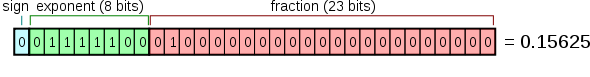
\includegraphics{32bit} \\[0.15cm]
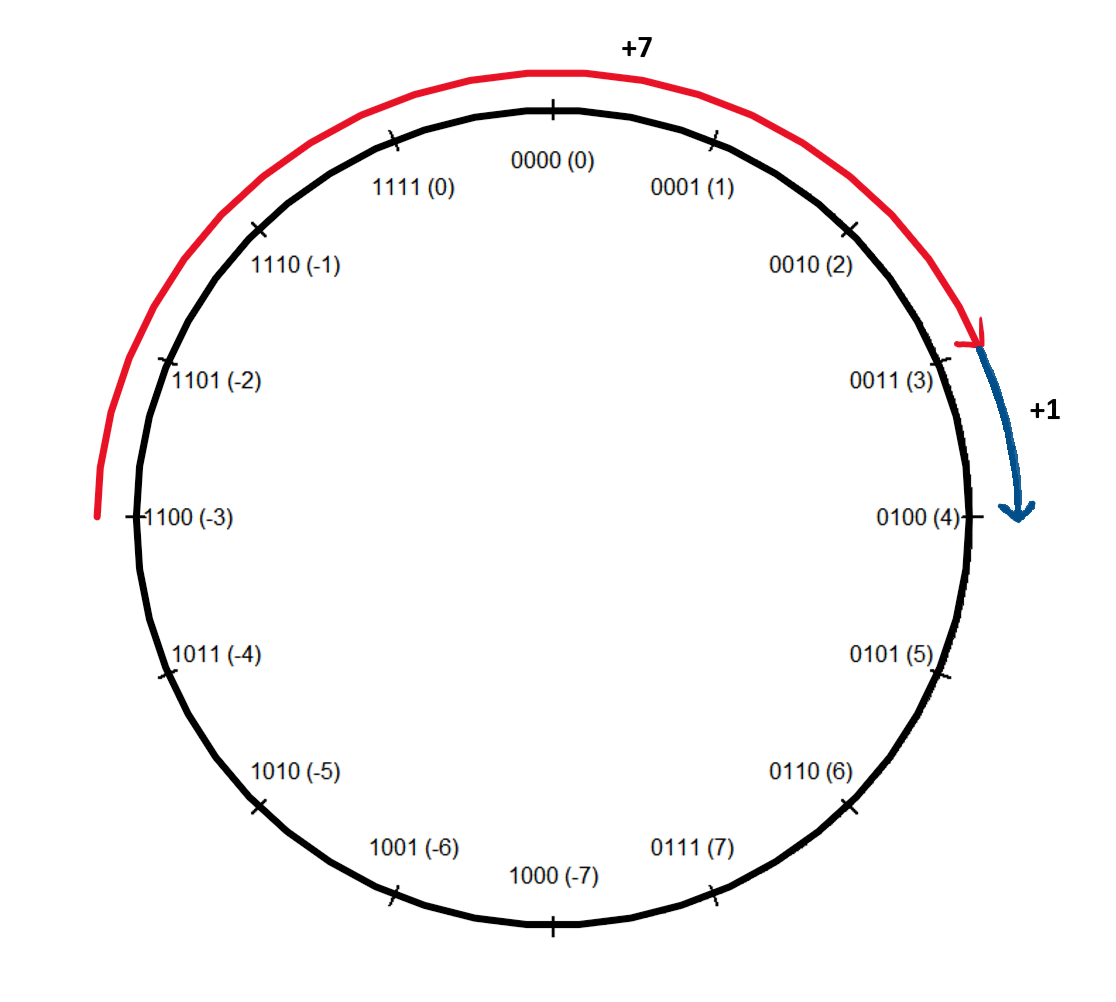
\includegraphics[width=0.4\paperwidth]{figure_man/1complement}
\end{tabular}
\end{center}

\vspace{-0.5cm}
\begin{itemize}
  \item Because of the $0$ being represented twice, a $1$ must be added when overflowing the $0$, so that the result is correct.
\end{itemize}

% <<>>=
% #1's complement
%  library(circular)
%  MyIntToBit <- function(x, dig) {
%      i <- 0L
%      string <- numeric(dig)
%      while (x > 0) {
%          string[dig - i] <- x %% 2L
%          x <- x %/% 2L
%          i <- i + 1L
%      }
%      string
%  }
%  y = lapply(0:(2^4 - 1), function(x) MyIntToBit(x,4))
%  y = lapply(y, function(x) paste(x, collapse = ""))
%  y = unlist(y)
%
%  y = paste(y, paste0("(", c(0:7, -7:-1, 0), ")"))
%
%  x = circular(seq(0, 2*pi - pi/8, pi/8))
%  plot(x, axes = FALSE, ticks = TRUE, type="n")
%  axis.circular(at=circular(seq(0, 2*pi - pi/8, pi/8), rotation = "clock", zero = 4 * pi/8),
%                labels = y, lwd = 2, tcl = 0.05)
%
% #2's complement
%  y = lapply(0:(2^4 - 1), function(x) MyIntToBit(x,4))
%  y = lapply(y, function(x) paste(x, collapse = ""))
%  y = unlist(y)
%
%  y = paste(y, paste0("(", c(0:7, -8:-1), ")"))
%
%  x = circular(seq(0, 2*pi - pi/8, pi/8))
%  plot(x, axes = FALSE, ticks = TRUE, type="n")
%  axis.circular(at=circular(seq(0, 2*pi - pi/8, pi/8), rotation = "clock", zero = 4 * pi/8),
%                labels = y, lwd = 2, tcl = 0.05)
%
% @

% \framebreak
%
% Allgemein
%
% \begin{eqnarray*}
%   \tilde x + x &=& \sum_{i=1}^{31} (u_i + \tilde u_i) 2^{i-1} - (u_{32} + \tilde u_{32})(2^{31} - 1)
% \end{eqnarray*}
%
% wobei
%
% $$
% (u_i + \tilde u_i) 2^{i-1}= \begin{cases}0 \cdot 2^{i-1} & \quad \text{wenn }u_i + \tilde u_i = 0 \\
% 1 \cdot 2^{i-1} & \quad \text{wenn }u_i + \tilde u_i = 1 \\
% 1 \cdot 2^{i} + 0 \cdot 2^{i-1} & \quad \text{wenn }u_i + \tilde u_i = 2 \text{ (Übertrag!)}
% \end{cases}
% $$

\end{vbframe}

\begin{vbframe}{Two's complement}

With the two's complement, negative numbers are formed by determining the one's complement and adding an additional 1.

\lz 

Example: conversion of $-51_{10}$:
\begin{footnotesize}
\begin{center}
  \begin{tabular}{ c | ccccccccccc}
      & \multicolumn{11}{c}{Bit $u_i$} \\
    %\cline{2-12}
      & 32 & 31  & $\hdots$ & 8 & 7 & 6 & 5 & 4 & 3 & 2 & 1 \\
    \hline
    $|-51_{10}|$  & 0 & 0 & $\hdots$ & 0 & 0 & 1 & 1 & 0 & 0 & 1 & 1 \\
    invert & 1 & 1 & $\hdots$ & 1 & 1 & 0 & 0 & 1 & 1 & 0 & 0 \\
    add 1 & 1 & 1 & $\hdots$ & 1 & 1 & 0 & 0 & 1 & 1 & 0 & 1 \\
    \hline
      & $-2^{31}$ & $2^{30}$ & $\hdots$ & $2^7$ & $2^6$ & $2^5$ & $2^4$ & $2^3$ & $2^2$ & $2^1$ & $2^0$
  \end{tabular}
\end{center}
\end{footnotesize}

\framebreak


Example: two's complement
\begin{footnotesize}
\begin{center}
  \begin{tabular}{ c | ccccccccccc}
      & \multicolumn{11}{c}{Bit $u_i$} \\
    %\cline{2-12}
      & 32 & 31  & $\hdots$ & 8 & 7 & 6 & 5 & 4 & 3 & 2 & 1 \\
    \hline
    $-2^{31}$    & 1 & 0 & $\hdots$ & 0 & 0 & 0 & 0 & 0 & 0 & 0 & 0 \\
    -51          & 1 & 1 & $\hdots$ & 1 & 1 & 0 & 0 & 1 & 1 & 0 & 1 \\
    -1           & 1 & 1 & $\hdots$ & 1 & 1 & 1 & 1 & 1 & 1 & 1 & 1 \\
    0            & 0 & 0 & $\hdots$ & 0 & 0 & 0 & 0 & 0 & 0 & 0 & 0 \\
    1            & 0 & 0 & $\hdots$ & 0 & 0 & 0 & 0 & 0 & 0 & 0 & 1 \\
    51           & 0 & 0 & $\hdots$ & 0 & 0 & 1 & 1 & 0 & 0 & 1 & 1 \\
    $2^{31}-1$   & 0 & 1 & $\hdots$ & 1 & 1 & 1 & 1 & 1 & 1 & 1 & 1 \\
    \hline
      & $-2^{31}$ & $2^{30}$ & $\hdots$ & $2^7$ & $2^6$ & $2^5$ & $2^4$ & $2^3$ & $2^2$ & $2^1$ & $2^0$
  \end{tabular}
\end{center}
\end{footnotesize}

The coded number is then: $x = \sum_{i=1}^{31} u_i 2^{i-1} - u_{32} 2^{31}$.

\framebreak
\begin{itemize}
\item Covered number range in 32-bit: $-2^{31}$ to $2^{31} - 1$
\item Not easy to read anymore. But big advantages for the computer.
\item Unique representation of $0$.
\item Addition / subtraction works as desired. As long as you stay in the number range, you can simply write and add two numbers below each other (the carry bit is ignored).
\end{itemize}
Example: $7 - 3$ in a 4-bit system:


\begin{center}
  \begin{tabular}{crl}
    &0111  &|(7)\\
    +&1101  &|(-3)\\\hline
    &(1)0100&|(4)
  \end{tabular}
\end{center}

\framebreak
The carry bit can simply be ignored here, since the representation of the $0$ is unique:

\vspace{-0.5cm}
\begin{center}
\begin{tabular}{l}
% $\,\,$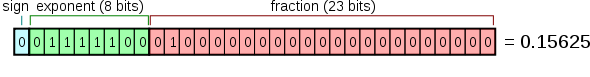
\includegraphics{32bit} \\[0.15cm]
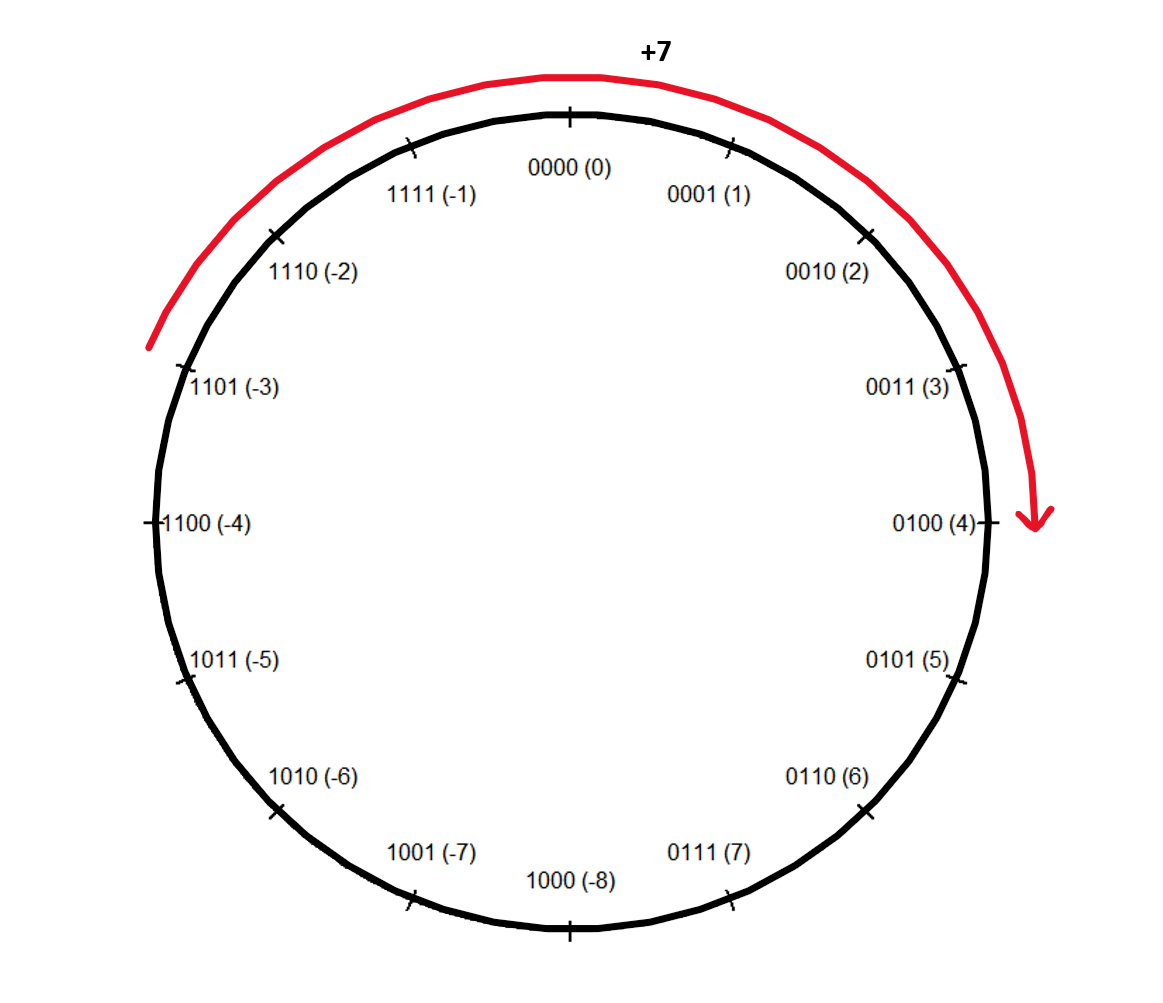
\includegraphics[width=0.4\paperwidth]{figure_man/2complement}
\end{tabular}
\end{center}

\vspace{-0.5cm}

\begin{itemize}
\item Caution when leaving the number range:
\item Example: $0011 \text{ (3)} + 0101 \text{ (5)} = 1000 \text{ (-8)}$
\end{itemize}

% \begin{center}
%   \begin{tabular}{crl}
%     &0011  &|(3)\\
%     +&0101  &|(5)\\\hline
%     &1000&|(-8)
%   \end{tabular}
% \end{center}


% \begin{itemize}
%   \item Wegen der doppelten Darstellung der 0 muss beim Überlaufen der 0 eine 1 addiert werden, damit das Ergebnis richtig ist.
% \end{itemize}

% In \pkg{R} erfolgt die Darstellung von ganzen Zahlen durch das 2er-Komplement.
%
% Positive Zahlen werden wie bisher in Bits konvertiert.
% Stehen 32 Bit zur Verfügung, wird das 32. Bit auf 0 gesetzt.
%
% Bei negativen Zahlen wird der Absolutbetrag in Bits konvertiert, dann alle Bits
% invertiert und eine 1 addiert (ohne Overflow). Dies hat immense Vorteile, da
% z.B. Addition, Subtraktion und Multiplikation für vorzeichenbehaftete Zahlen
% prinzipiell genauso wie für Zahlen ohne Vorzeichen ausgeführt werden können.
%

%

%
%

%
% Abgedeckter Zahlenbereich: $-2^{31}$ bis $2^{31} - 1$.
% <<>>=
% print(.Machine$integer.max)
% @


\end{vbframe}

\begin{vbframe}{Integer Overflow}

\textbf{Caution:} Arithmetic operations can cause an \textbf{overflow}.
This is a common programming error in languages like C and can lead to undefined behavior (e.g. wrap around).

\lz

\textbf{Example}: $(2^{31} - 1) + 1$.

In a 32-bits two's complement representation $(2^{31} - 1) + 1$ would be outside of the covered number range, since $(2^{31} - 1)$ is the largest possible number that can be represented. Adding $1$ results in $-2^{31}$ due to an integer overflow.

\lz 

\centering
\begin{tabular}{c:cccc}
$(2^{31} - 1)$ & 01111111 & 11111111 & 11111111 & 11111111 \\
$+ 1$ & 00000000 & 00000000 & 00000000 & 00000001 \\
\hline
$(-2^{31})$ & 10000000 & 00000000 & 00000000 & 00000000 \\
\end{tabular}

\framebreak

Excerpt from Wikipedia \enquote{Integer Overflow}:

\lz

\emph{
On 30 April 2015, the Federal Aviation Authority announced it will order Boeing 787 operators to reset its electrical system periodically, to avoid an integer overflow which could lead to loss of electrical power and ram air turbine deployment, and Boeing is going to deploy a software update in the fourth quarter.}

\lz

\emph{When Donkey Kong breaks on level 22 it is because of an integer overflow in its time/bonus. Donkey Kong takes the level number you're on, multiplies it by 10 and adds 40. When you reach level 22 the time/bonus number is 260 which is too large for its 8-bit 256 value register so it resets itself to 0 and gives the remaining 4 as the time/bonus - not long enough to complete the level.}


\end{vbframe}

\begin{vbframe}{Machine numbers for $\Z$ in \pkg{R}}

In \pkg{R}, integers are encoded in 32-bit (also in 64-bit \pkg{R}!) by the two's complement. 

\footnotesize
\vspace{0.5cm}
\begin{verbbox}
.Machine$integer.max
## [1] 2147483647
\end{verbbox}
\col
\vspace{0.2cm}
\begin{verbbox}
2^31 - 1
## [1] 2147483647
\end{verbbox}
\col

\framebreak 

\footnotesize
\vspace{0.5cm}
\begin{verbbox}
intToBits(-51L)
## [1] 01 00 01 01 00 00 01 01 01 01 01 01 01 01 01 01 01 01
## [19] 01 01 01 01 01 01 01 01 01 01 01 01 01 01
\end{verbbox}
\col
\vspace{0.2cm}
\begin{verbbox}
intToBits(51L)
## [1] 01 01 00 00 01 01 00 00 00 00 00 00 00 00 00 00 00 00
## [19] 00 00 00 00 00 00 00 00 00 00 00 00 00 00
\end{verbbox}
\col
\vspace{0.2cm}
\begin{verbbox}
# Caution: In R the operation x^y always results in the type 'numeric'!
intToBits(2L^31L - 1L)
## [1] 01 01 01 01 01 01 01 01 01 01 01 01 01 01 01 01 01 01
## [19] 01 01 01 01 01 01 01 01 01 01 01 01 01 00
\end{verbbox}
\col


\framebreak 
\normalsize
In \pkg{R}, integer overflows are caught and set to NA.
\lz
\footnotesize
\begin{verbbox}
.Machine$integer.max + 1 
## [1] 2147483648
\end{verbbox}
\col
\vspace{0.2cm}
\begin{verbbox}
str(.Machine$integer.max + 1) 
## num 2.15e+09
\end{verbbox}
\col
\vspace{0.2cm}
\begin{verbbox}
str(.Machine$integer.max + 1L)
## Warning in .Machine$integer.max + 1L: NAs produced by 
   integer overflow
## int NA
\end{verbbox}
\col

\end{vbframe}
\normalsize

\begin{vbframe}
\frametitle{R in 64-bit systems}
\begin{itemize}
  \item In 2010, the 64-bit version of R was released.
  \item \textbf{But:} integers are still encoded in 32-bit.
  \item The largest integer in R is thus about 2 billion.
  \item When indexing vectors longer than about 2 billion, R uses a trick:
  \begin{itemize}
    \item By using floating point numbers in double precision, integers can be represented reliably within the value range $(-2^{53}, 2^{53})$.
    \item Beyond that, not all integers are covered!
    \item In R you can index with floating point numbers:
  \end{itemize}
\end{itemize}

\footnotesize
\lz
\begin{verbbox}
c(1,2,3)[1.7]
## [1] 1
\end{verbbox}
\col
\end{vbframe}



\endlecture
\end{document}

% https://github.com/SurajGupta/r-source/blob/56becd21c75d104bfec829f9c23baa2e144869a2/src/library/stats/src/cov.c

